\section{Photometric Value Calculation}
%Výpočet mnohonásobných odrazů, algoritmus - odrazy
To evaluate the lighting system's quality of the model room in terms of standard \cite{12464} four parameters have to be observed listed in section \ref{sec:design}. For simplification reasons parameter $UGR_{L}$ will not be calculated. $R_{a}$ is a parameter of the chosen luminaire and is not affected by the model room. Uniformity $U_{0}$ is calculated by the following equation:

\begin{equation}
U_{0}=\frac{E_{min}}{\overline{E}} \quad \mathrm{(-;lx,lx)}
\end{equation}

where:
\begin{description}
	\item[$E_{min}$] is the minimum illuminance of the working plane,
	\item[$\overline{E}$] is the average illuminance of the working plane.
\end{description}

Illuminances can be acquired by measurements or calculations in certain points of working planes that are chosen in accordance to the purpose of the room. To calculate the illuminance in a given point of the working plane contributions of all light sources illuminating the given point have to be summed up. This can be achieved by using luminous intensities of all the light sources pointing from the light source towards the point (as seen in figure \ref{fig:osv}):

\begin{equation}
E_{P\rho}=\sum_{i} \frac{I_{C \gamma i} \cdot \cos{\beta_{i}}}{{l_{i}}^{2}}
\end{equation}

where:
\begin{description}
	\item[$I_{C \gamma i}$] is the luminous intensity of the light source pointing towards point P of plane $\rho$,
	\item[$\beta_{i}$] is the angle between the normal of plane $\rho$ and the light ray from light source $S_{i}$,
	\item[$\l_{i}$] is the distance of point $P$ from the light source.
\end{description}

\begin{figure}[htb] \label{fig:osv}
  \centering
  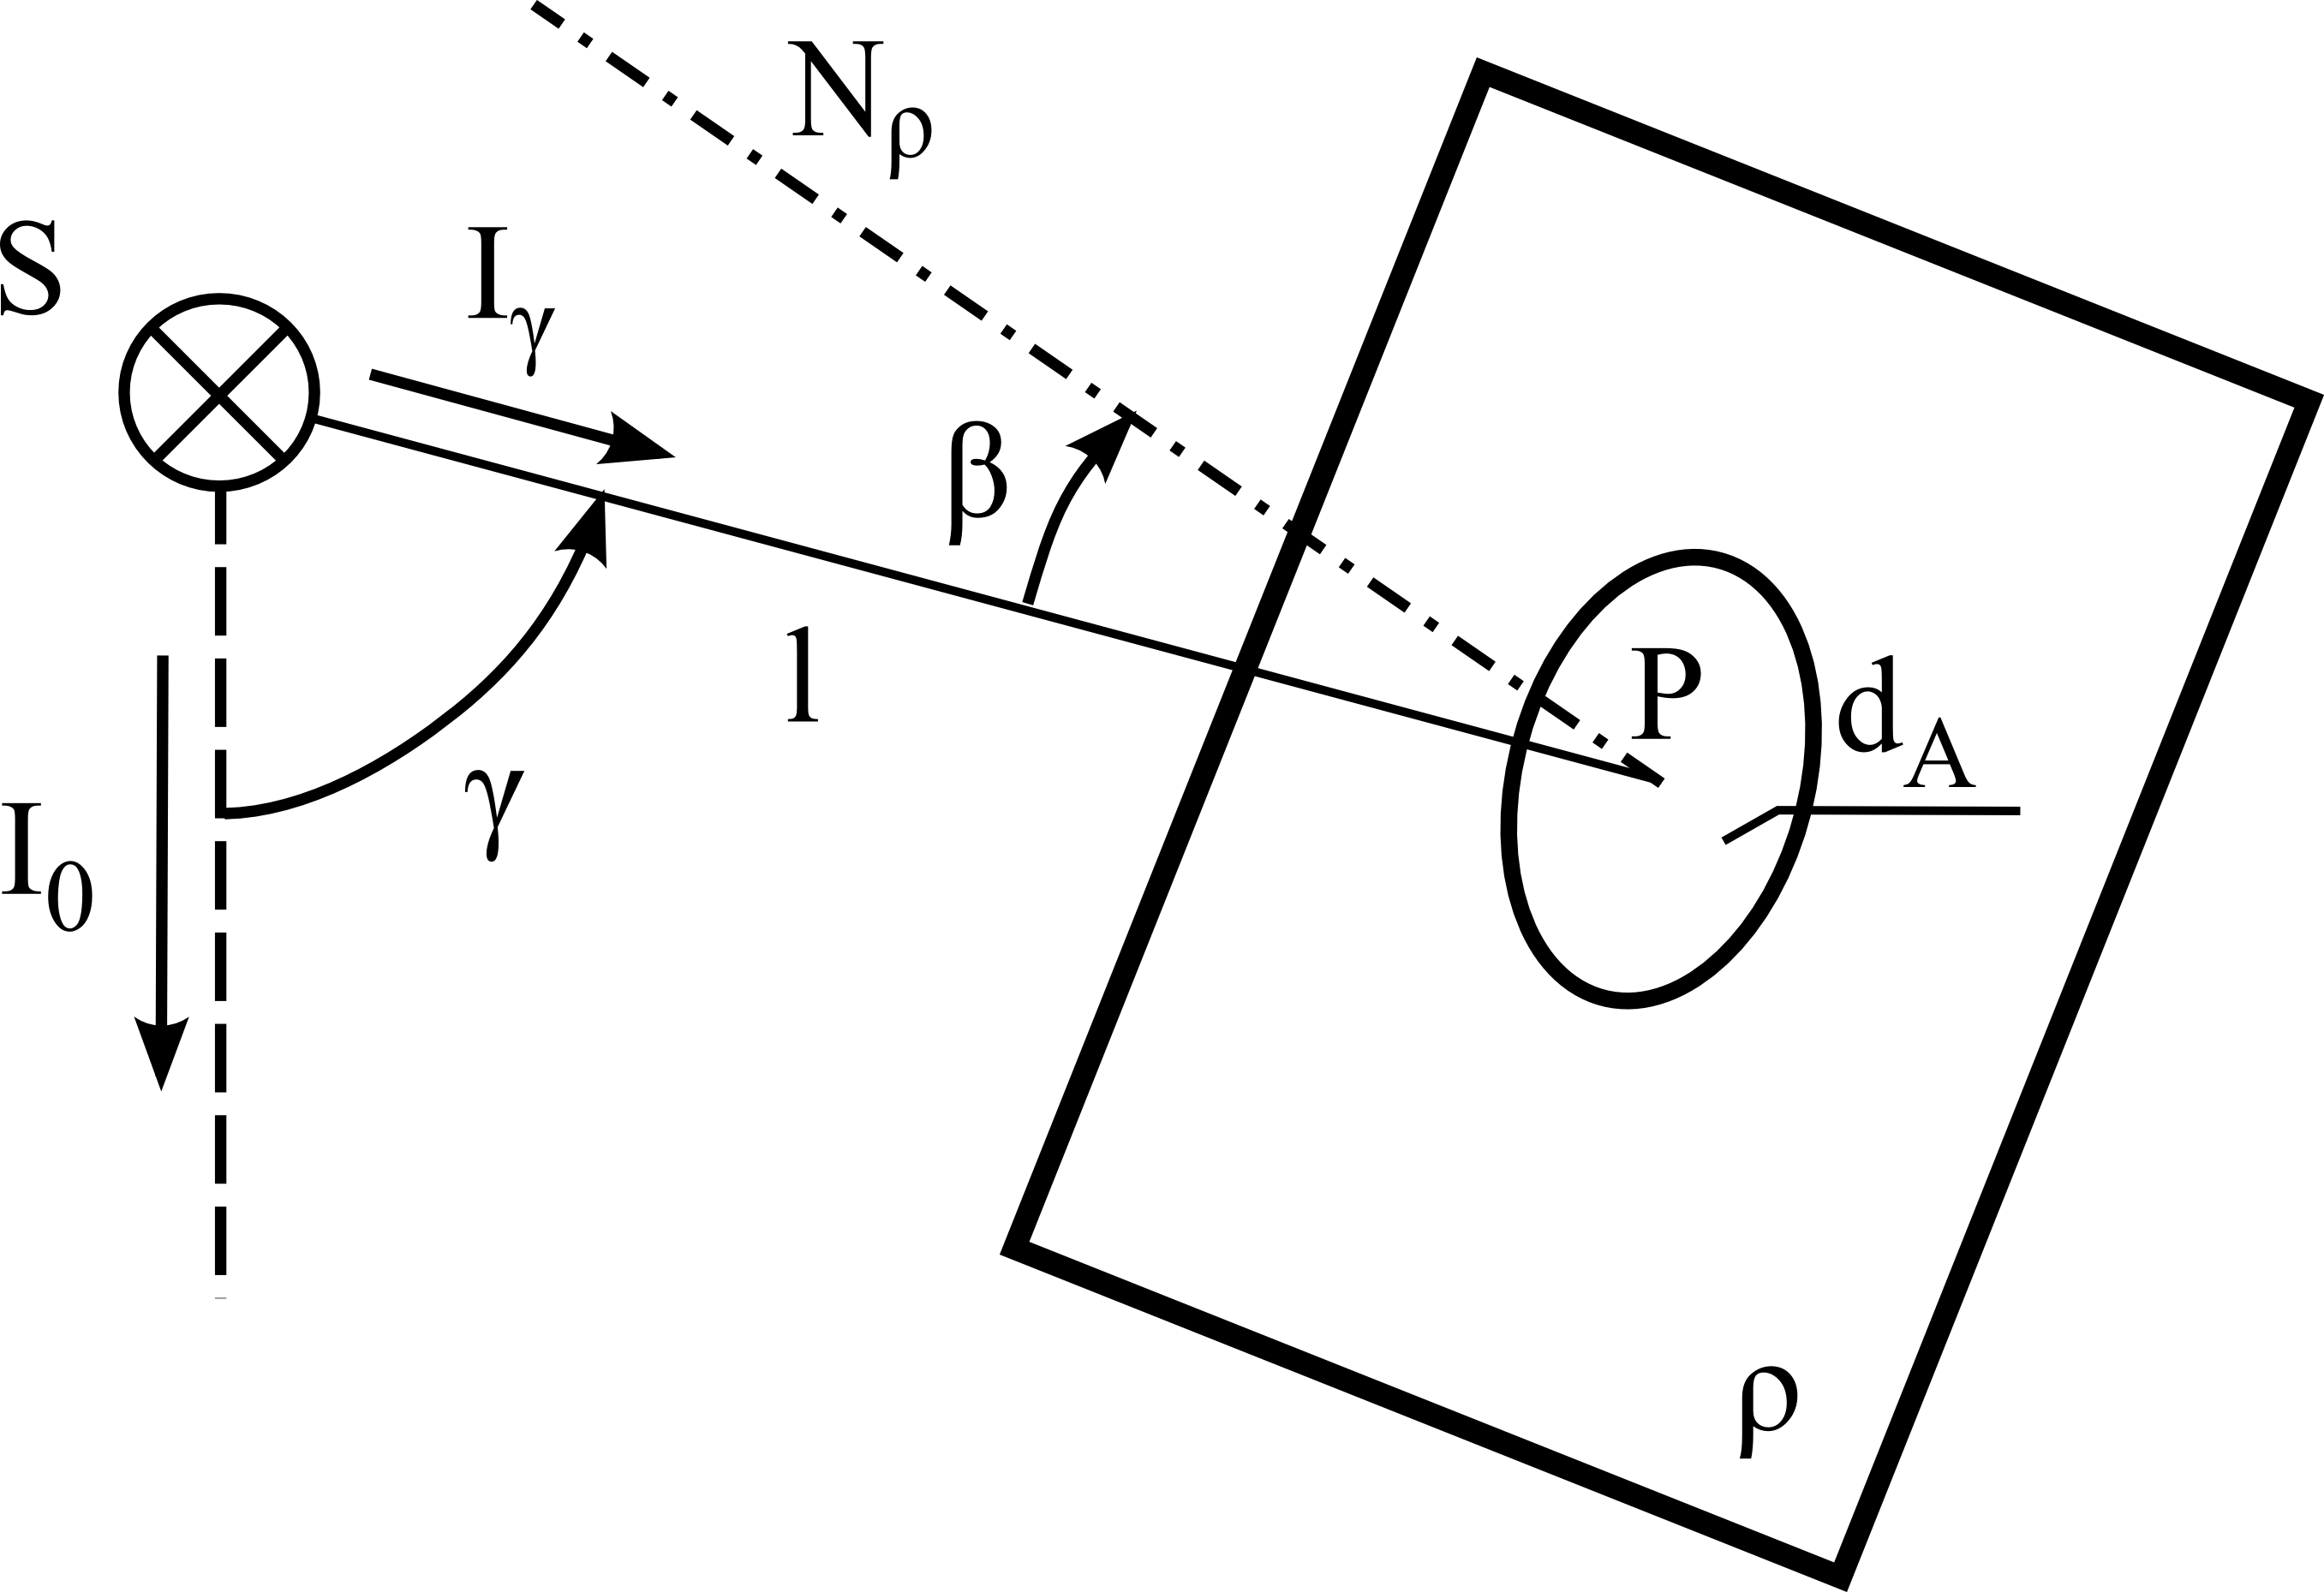
\includegraphics[width=\columnwidth]{315_osvetlenost_bodovym_zdrojem}
  \caption{Graphs of parts $g_1\left(E_{avg}\right)$ and $g_2\left(U_0\right)$ from the fitness function}
\end{figure}


 luminous intensities of all light sources illuminating the point have to be summed up.
luminous flux incident on the working plane in the close proximity of the point has to be acquired. Illuminances can be calculated by the following equation:

\begin{equation}
E=\frac{\mathrm{d}\Phi}{\mathrm{d}A} \quad \mathrm{(lx;lm,m^{2})}
\end{equation}





The average illuminance $E$ of a planar surface is the areal density of luminous flux incident on the surface \cite{Habel}:

\begin{equation} \label{eq:illuminance}
E=\frac{d\Phi_{i}}{dA} \quad \mathrm{(lx;lm,m^2)}
\end{equation}

where:
\begin{description}
	\item[$d\Phi_{i}$] is the luminous flux incident on a surface,
	\item[$dA$] is the surface area.
\end{description}

